\subsection{Experimental Setup}
\label{sec:setup}

\subsubsection{System used}

We experiment on a system consisting of a $64$-core x86-based AMD EPYC-7742 processor running at $2.25$ GHz. Each core has an L1 cache of $4$ MB, an L2 cache of $32$ MB, and a shared L3 cache of $256$ MB. The server has $512$ GB DDR4 system memory, and runs on Ubuntu $20.04$.


\subsubsection{Configuration}

We use 32-bit integers for vertex ids and 64-bit floating point numbers for vertex ranks. To mark vertices as affected, we use an 8-bit integer vector. The rank computation uses OpenMP's \textit{dynamic schedule} with a chunk size of $2048$, which provides dynamic work-balancing among threads. We use a damping factor of $\alpha = 0.85$ \cite{rank-langville06}, an iteration tolerance of $\tau = 10^{-10}$ \cite{rank-dubey22} using $L\infty$-norm \cite{rank-plimpton11}, and limit the \texttt{MAX\_ITERATIONS} performed to $500$ \cite{nvgraph} for all experiments. We run all experiments with $64$ threads to match the number of cores available on the system (unless specified otherwise). For compilation, we use GCC $9.4$ and OpenMP $5.0$.


\subsubsection{Dataset}

We use four classes of graphs from the \textit{SuiteSparse Matrix Collection} \cite{suite19} in our experiments, shown in Table \ref{tab:dataset}. The number of vertices in these graphs varies from $3.07$ million to $214$ million, and the number of edges varies from $37.4$ million to $1.98$ billion. The presence of dead ends (vertices with no out-links) introduces a global teleport rank contribution that must be computed every iteration. We eliminate this overhead by adding self-loops to all the vertices in the graph (see also \cite{rank-andersen07, rank-langville06}).
%% We also use temporal graph for certain experiments, mention here?

\begin{table}[hbtp]
  \centering
  \caption{List of 12 graphs obtained SuiteSparse Matrix Collection \cite{suite19} (directed graphs are marked with $*$). Here, $|V|$ is the number of vertices, $|E|$ is the number of edges (after adding self-loops), and $D_{avg}$ is the average degree.\ignore{, and $\Gamma_G$ is the Gini coefficient of PageRank distribution. In the table, B refers to a billion, M refers to a million and K refers a thousand.}}
  \label{tab:dataset}
  \begin{tabular}{|c||c|c|c|c|}
    \toprule
    \textbf{Graph} &
    \textbf{\textbf{$|V|$}} &
    \textbf{\textbf{$|E|$}} &
    \textbf{\textbf{$D_{avg}$}} \\
    % \textbf{$1 - \Gamma_G$} \\
    \midrule
    \multicolumn{4}{|c|}{\textbf{Web Graphs (LAW)}} \\ \hline
    indochina-2004$^*$ & 7.41M & 199M & 26.8 \\ \hline  % & \num{4.7e-4}
    % uk-2002$^*$ & 18.5M & 311M & 16.8 \\ \hline  % & \num{9.6e-5}
    arabic-2005$^*$ & 22.7M & 654M & 28.8 \\ \hline  % & \num{5.5e-4}
    uk-2005$^*$ & 39.5M & 961M & 24.3 \\ \hline  % & \num{9.6e-5}
    webbase-2001$^*$ & 118M & 1.11B & 9.4 \\ \hline  % & \num{7.3e-7}
    it-2004$^*$ & 41.3M & 1.18B & 28.5 \\ \hline  % & \num{3.8e-4}
    sk-2005$^*$ & 50.6M & 1.98B & 39.1 \\ \hline  % & \num{5.8e-4}
    \multicolumn{4}{|c|}{\textbf{Social Networks (SNAP)}} \\ \hline
    com-LiveJournal & 4.00M & 73.4M & 18.3 \\ \hline  % & \num{7.9e-4}
    com-Orkut & 3.07M & 237M & 77.3 \\ \hline  % & \num{6.7e-2}
    \multicolumn{4}{|c|}{\textbf{Road Networks (DIMACS10)}} \\ \hline
    asia\_osm & 12.0M & 37.4M & 3.1 \\ \hline  % & \num{8.4e-4}
    europe\_osm & 50.9M & 159M & 3.1 \\ \hline  % & \num{6.6e-4}
    \multicolumn{4}{|c|}{\textbf{Protein k-mer Graphs (GenBank)}} \\ \hline
    kmer\_A2a & 171M & 531M & 3.1 \\ \hline  % & \num{9.4e-5}
    kmer\_V1r & 214M & 679M & 3.2 \\ \hline  % & \num{3.2e-4}
  \bottomrule
  \end{tabular}
\end{table}



\subsubsection{Batch Generation}
\label{sec:batch-generation}

%% This needs to be updated
We take each base (static) graph from the dataset and generate a random batch update consisting of an equal mix of edge deletions and insertions. To prepare the set of edges deleted, we delete each existing edge with a uniform probability. We prepare the set of edges to insert by choosing pairs of vertices with equal probability. For the sake of simplicity, we ensure that no new vertices are added to or removed from the graph. We measure the batch size as a fraction of the total number of edges in the original graph and adjust it from $10^{-8}$ to $0.1$ (i.e., $10^{-8}|E|$ to $0.1|E|$), and generate multiple batches for each batch size (for averaging). Along with each batch update, we add self-loops to all vertices.


\subsubsection{Measurement}
\label{sec:measurement}

We measure the time taken by each approach on the updated graph entirely, including any preprocessing cost and the time taken to detect convergence, but exclude time taken for memory allocation and de-allocation. The average time taken by a given method at a given batch size is obtained by taking the geometric mean of time taken for the same batch size for each of the different input graphs. Accordingly, the average speedup is the ratio of these. Further, we measure the error/accuracy of a given approach by measuring the $L\infty$-norm of the ranks produced with respect to ranks obtained from a reference \textit{Static With-barrier} PageRank run on the updated graph with a very low tolerance of $\tau = 10^{-100}$ (limited to $500$ iterations).




\subsection{Performance of DF-PageRank}

We first study the performance of \FroWbar{} and \FroBarf{}  on batch updates of size $10^{-8} |E|$ to $0.1 |E|$, in the absence of faults, and compare them with \StaWbar{}, \StaBarf{}, \NaiWbar{}, and \NaiBarf{}. Figure \ref{fig:no-failure} plots the runtime of the six mentioned approaches. In Figure \ref{fig:no-failure}, solid lines represent the runtime of the barrier-free algorithms and dashed lines represent the runtime of the corresponding algorithms using a barrier. In addition to the runtime of the above algorithms on each instance from Table \ref{tab:dataset} shown in Figure \ref{fig:no-failure-all}, the mean runtime of each algorithm is shown in Figure \ref{fig:no-failure-am-time}. The labels on the line corresponding to \FroBarf{} indicate its speedup over \NaiBarf{}.

In Figure \ref{fig:no-failure-am-time}, we demonstrate that our proposed \FroBarf{}  is faster than \NaiBarf{} until a batch size of $10^{-3} |E|$, with an average speedup of $4.6\times$. From a batch size of $10^{-3} |E|$ (a batch update consisting of more than a million edge deletions / insertions on a billion-edge graph), the performance drops below \NaiBarf{} and \StaBarf{}. Such large batch sizes result in {\em nearly} all of the vertices getting marked as {\em affected}, and hence the performance drops. Note in Figure \ref{fig:no-failure-all} that \FroBarf{} performs well on \textit{road networks} and \textit{protein k-mer graphs}, good enough on \textit{web graphs}, but poorly on \textit{social networks}. This seems to be associated to sparsity of the graphs as \FroBarf{} performing well on sparse graphs.

\begin{figure*}[hbtp]
  \centering
  % \includegraphics[width=0.44\linewidth]{out/insertions-runtime-key.pdf}
  \subfigure[Overall result]{
    \label{fig:insertions-runtime--mean}
    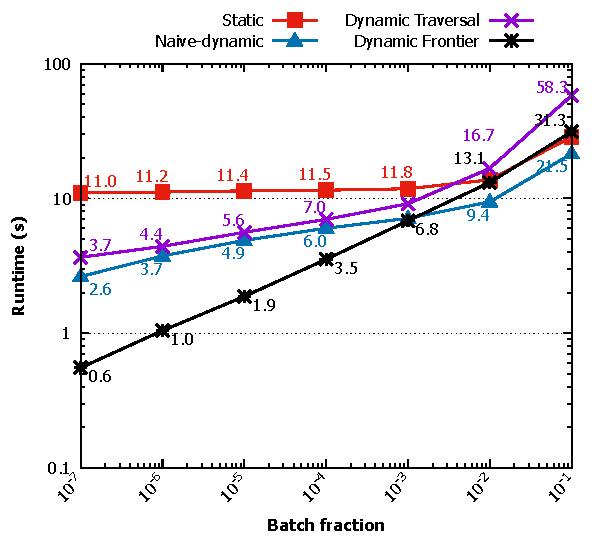
\includegraphics[width=0.38\linewidth]{out/insertions-runtime-mean.pdf}
  }
  \subfigure[Results on each graph]{
    \label{fig:insertions-runtime--all}
    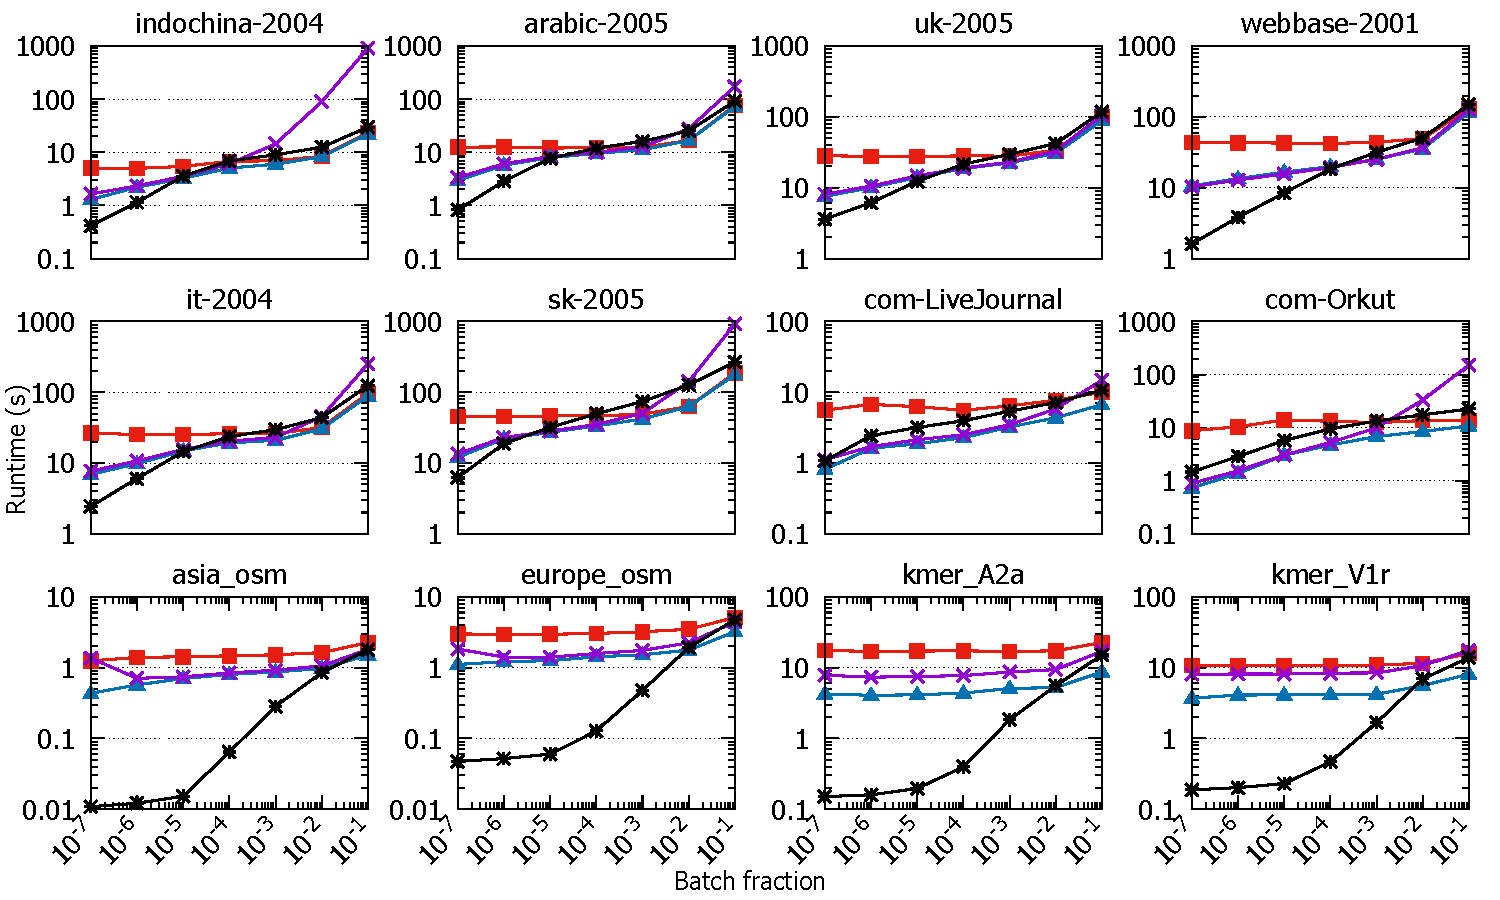
\includegraphics[width=0.58\linewidth]{out/insertions-runtime-all.pdf}
  } \\[-1ex]
  \caption{Runtime (logarithmic scale) for \textit{Static}, \textit{Naive-dynamic}, \textit{Dynamic Traversal}, and \textit{Dynamic Frontier} PageRank with batch updates exclusively comprising edge insertions, ranging from $10^{-7} |E|$ to $0.1 |E|$ in multiples of $10$ (logarithmic scale). The right figure details the runtime of each approach for individual graphs in the dataset, while the left figure displays overall runtimes --- using geometric mean for consistent scaling across graphs.}
  \label{fig:insertions-runtime}
\end{figure*}

\begin{figure*}[hbtp]
  \centering
  % \includegraphics[width=0.44\linewidth]{out/insertions-speedup-key.pdf}
  \subfigure[Overall result]{
    \label{fig:insertions-speedup--mean}
    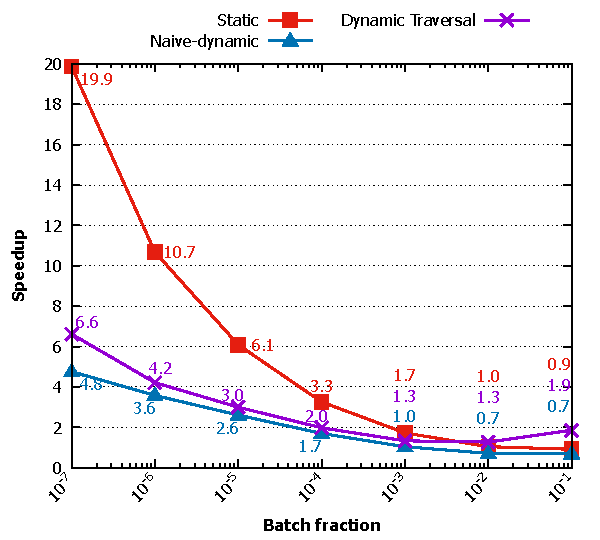
\includegraphics[width=0.38\linewidth]{out/insertions-speedup-mean.pdf}
  }
  \subfigure[Results on each graph]{
    \label{fig:insertions-speedup--all}
    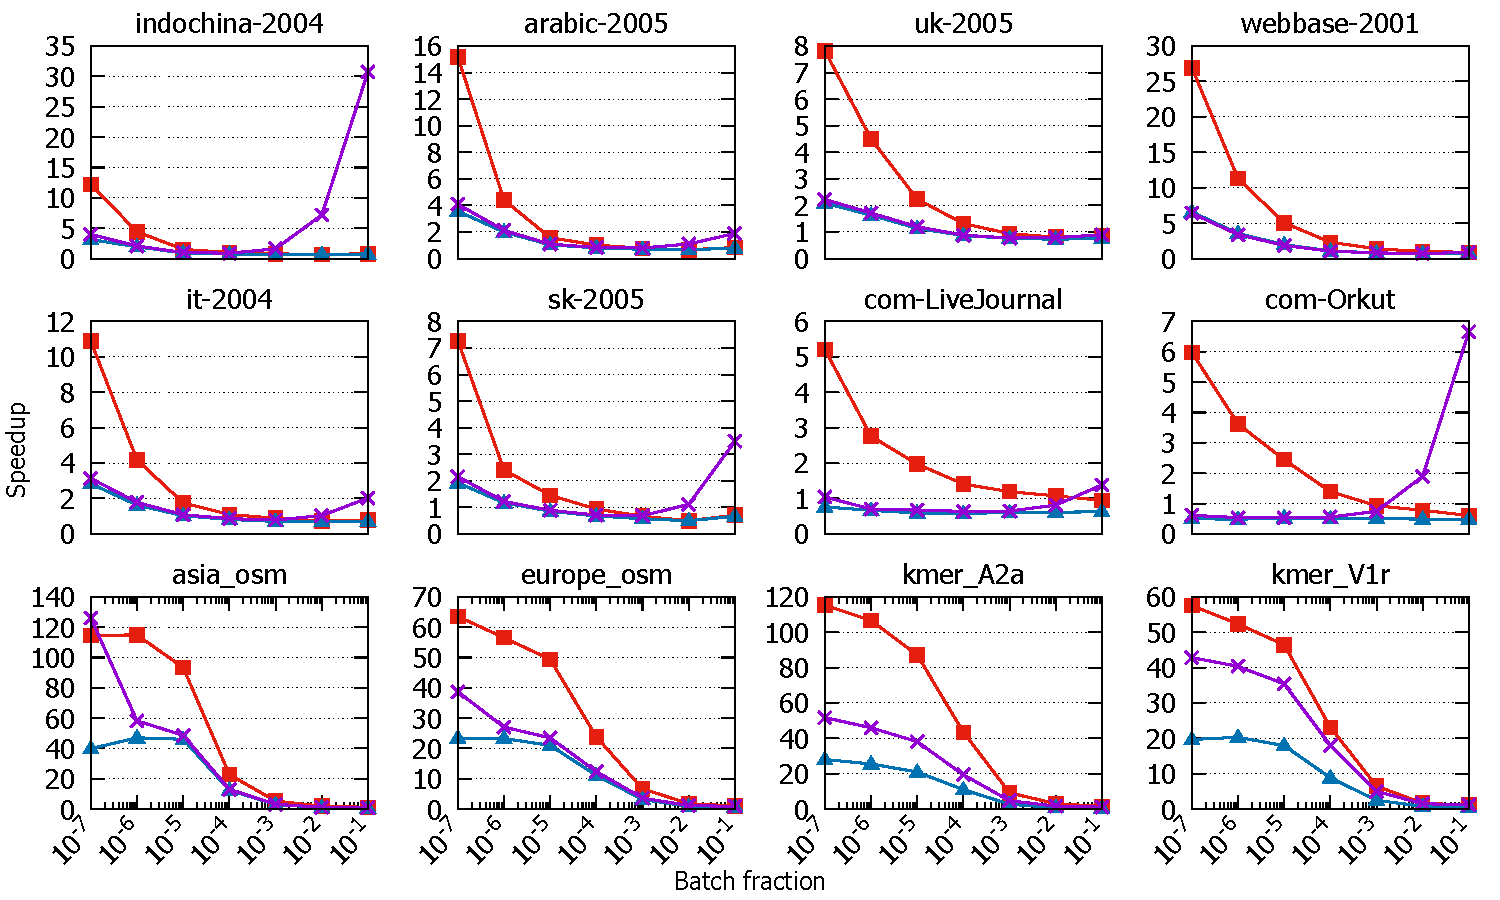
\includegraphics[width=0.58\linewidth]{out/insertions-speedup-all.pdf}
  } \\[-1ex]
  \caption{Speedup of \textit{Dynamic Frontier} PageRank with respect to \textit{Static}, \textit{Naive-dynamic}, and \textit{Dynamic Traversal} PageRank, on batch updates consisting solely of edge insertions ranging from $10^{-7} |E|$ to $0.1 |E|$ (logarithmic scale). The right figure depicts the speedup of \textit{Dynamic Frontier} PageRank in relation to each approach for individual graphs in the dataset, while the left figure highlights the overall speedup.}
  \label{fig:insertions-speedup}
\end{figure*}

\begin{figure*}[hbtp]
  \centering
  % \includegraphics[width=0.44\linewidth]{out/insertions-error-key.pdf}
  \subfigure[Overall result]{
    \label{fig:insertions-error--mean}
    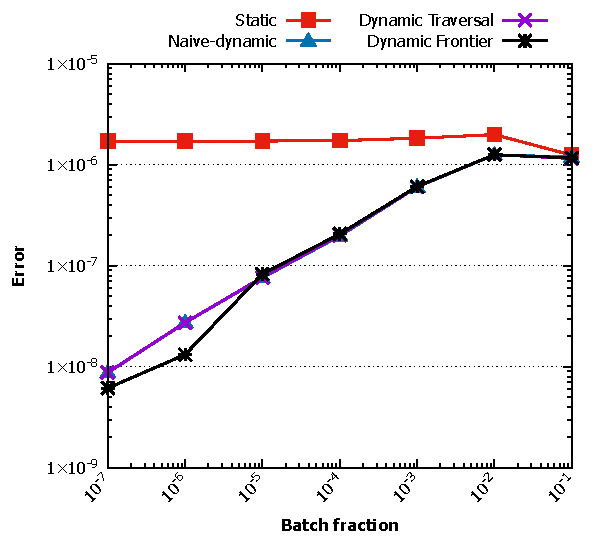
\includegraphics[width=0.38\linewidth]{out/insertions-error-mean.pdf}
  }
  \subfigure[Results on each graph]{
    \label{fig:insertions-error--all}
    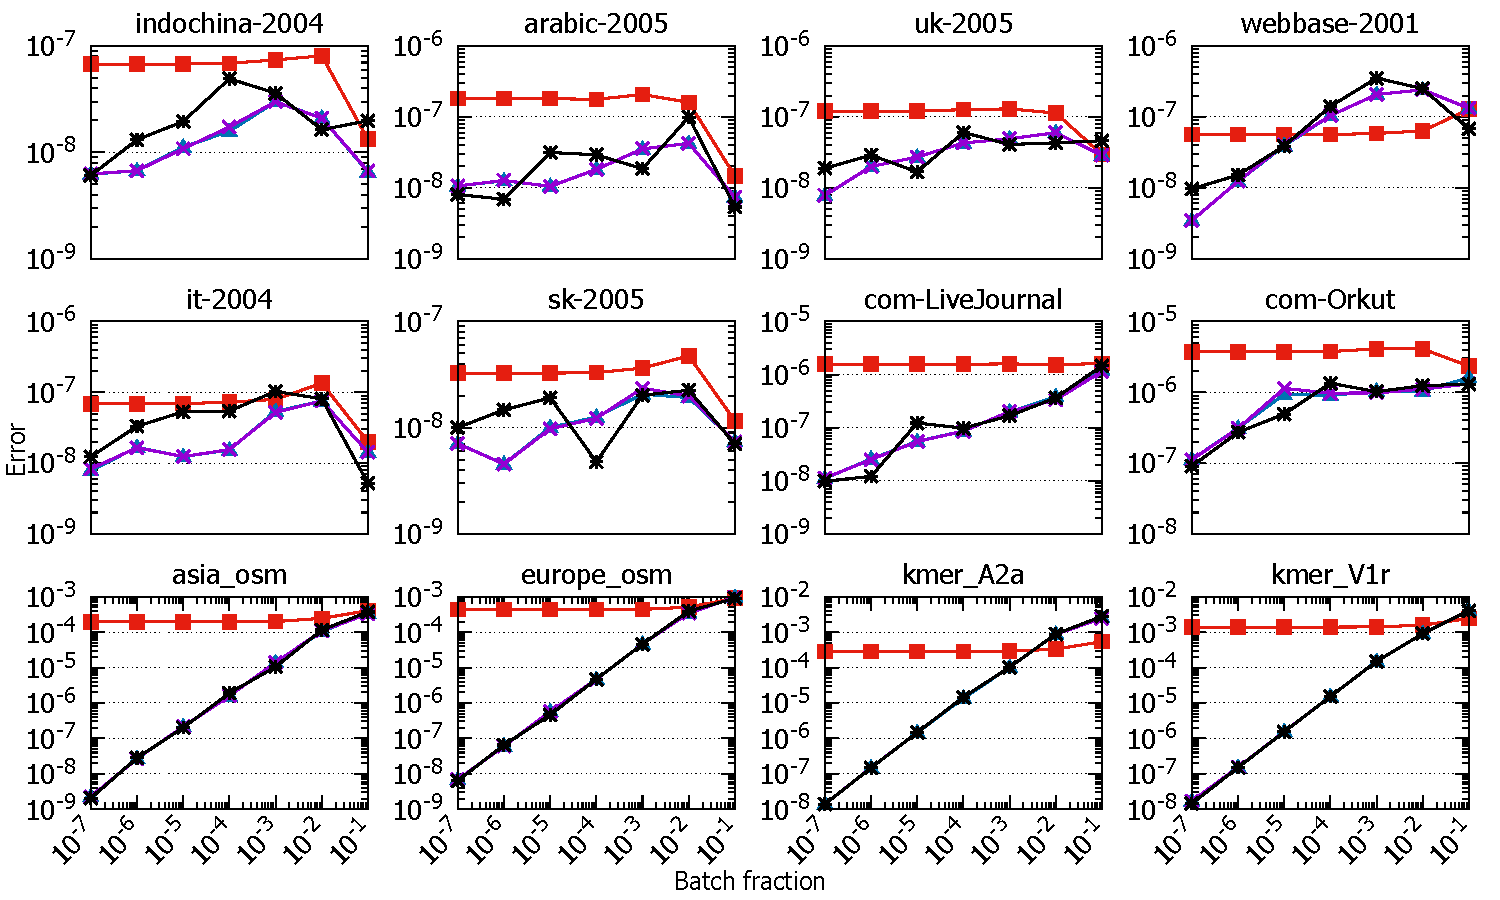
\includegraphics[width=0.58\linewidth]{out/insertions-error-all.pdf}
  } \\[-1ex]
  \caption{Error analysis comparing \textit{Static}, \textit{Naive-dynamic}, \textit{Dynamic Traversal}, and \textit{Dynamic Frontier} PageRank with a Reference Static PageRank (with a tolerance $\tau$ of $10^{-100}$ and limited to $500$ iterations) using $L1$-norm. Batch updates involve edge insertions ranging from $10^{-7} |E|$ to $0.1 |E|$ (logarithmic scale). The right figure illustrates the error specific to each approach for individual graphs in the dataset, while the left figure presents overall errors using the geometric mean for consistent scaling across graphs.}
  \label{fig:insertions-error}
\end{figure*}

\begin{figure*}[hbtp]
  \centering
  % \includegraphics[width=0.44\linewidth]{out/deletions-runtime-key.pdf}
  \subfigure[Overall result]{
    \label{fig:deletions-runtime--mean}
    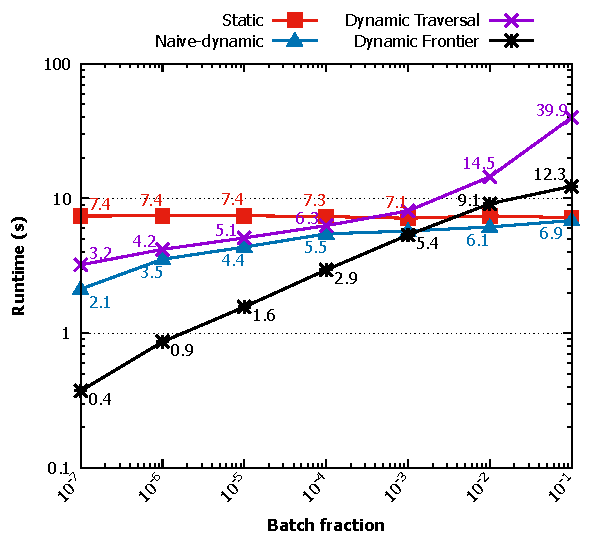
\includegraphics[width=0.38\linewidth]{out/deletions-runtime-mean.pdf}
  }
  \subfigure[Results on each graph]{
    \label{fig:deletions-runtime--all}
    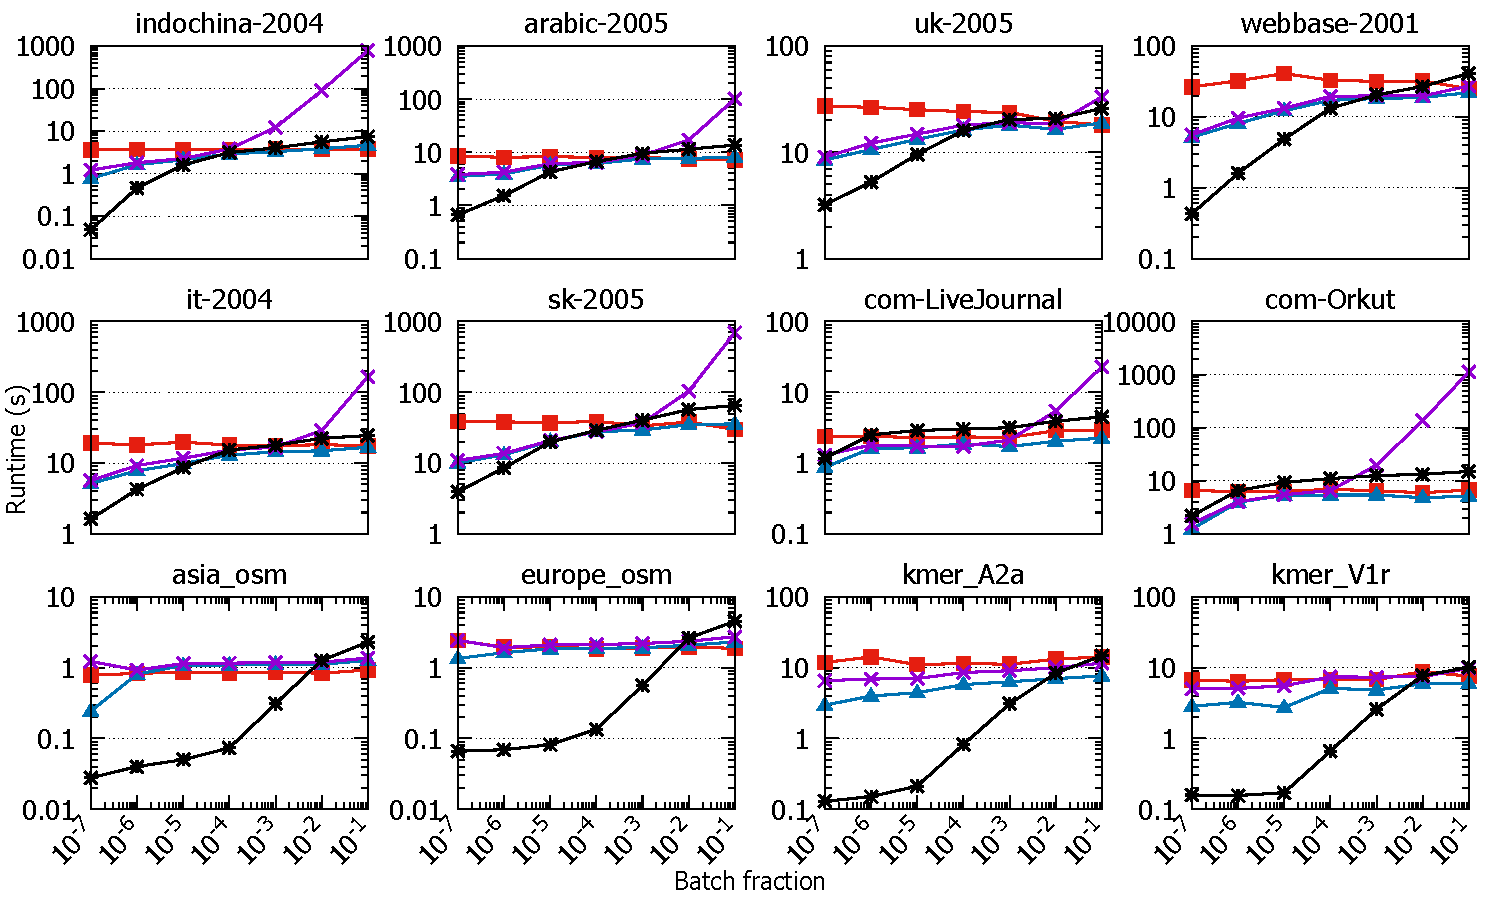
\includegraphics[width=0.58\linewidth]{out/deletions-runtime-all.pdf}
  } \\[-1ex]
  \caption{Deletions Time taken (solid lines), and modularity of communities obtained (dashed lines) along the Y2 axis, with X, X, and X (Algorithm X) on batch updates of increasing size from $10^{-7} |E|$ to $0.1 |E|$. Note that both axes are logarithmic. The numbers on the lines corresponding to X and X indicate the speedup of X over  the two algorithms, respectively.}
  \label{fig:deletions-runtime}
\end{figure*}

\begin{figure*}[hbtp]
  \centering
  % \includegraphics[width=0.44\linewidth]{out/deletions-speedup-key.pdf}
  \subfigure[Overall result]{
    \label{fig:deletions-speedup--mean}
    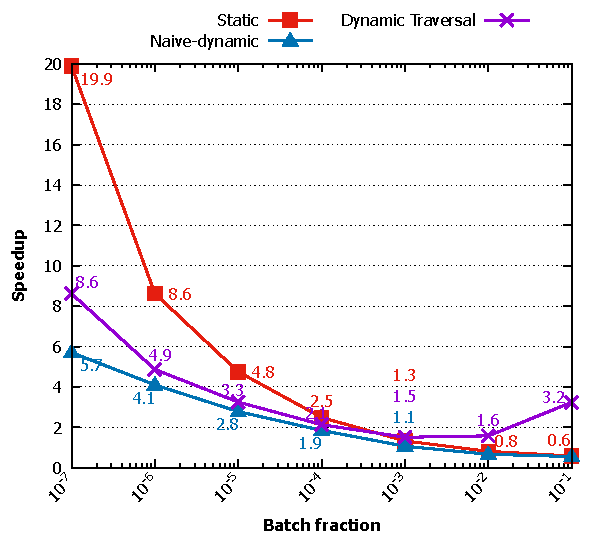
\includegraphics[width=0.38\linewidth]{out/deletions-speedup-mean.pdf}
  }
  \subfigure[Results on each graph]{
    \label{fig:deletions-speedup--all}
    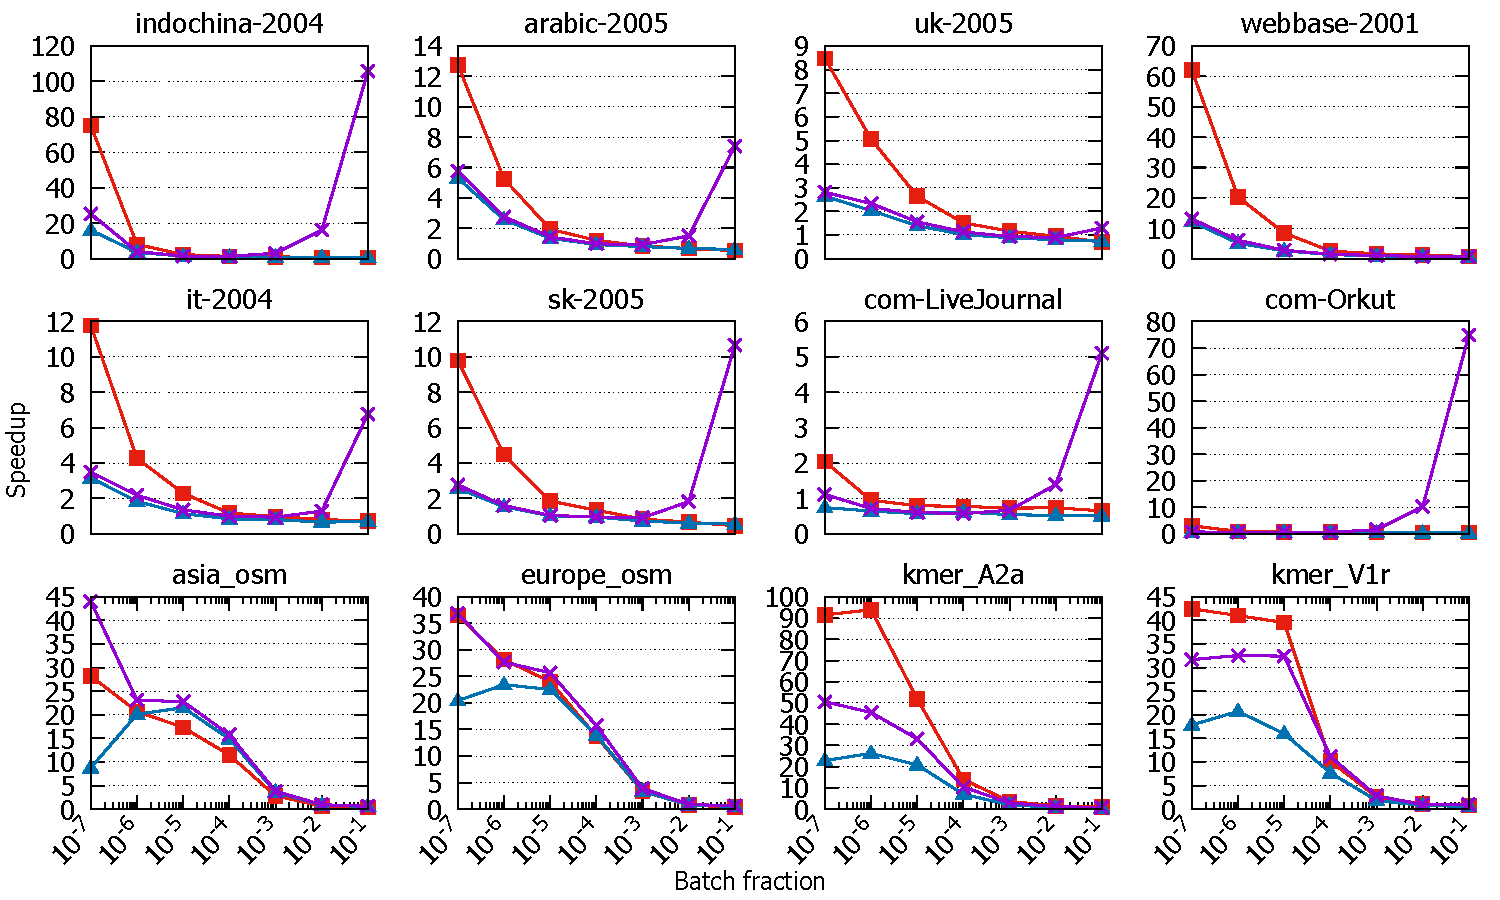
\includegraphics[width=0.58\linewidth]{out/deletions-speedup-all.pdf}
  } \\[-1ex]
  \caption{Speedup of \textit{Dynamic Frontier} PageRank in relation to \textit{Static}, \textit{Naive-dynamic}, and \textit{Dynamic Traversal} PageRank, on batch updates comprised solely of edge deletions ranging from $10^{-7} |E|$ to $0.1 |E|$ (logarithmic scale). The right figure illustrates the speedup of \textit{Dynamic Frontier} PageRank concerning each approach for individual graphs in the dataset, while the left figure emphasizes the overall speedup.}
  \label{fig:deletions-speedup}
\end{figure*}

\begin{figure*}[hbtp]
  \centering
  % \includegraphics[width=0.44\linewidth]{out/deletions-error-key.pdf}
  \subfigure[Overall result]{
    \label{fig:deletions-error--mean}
    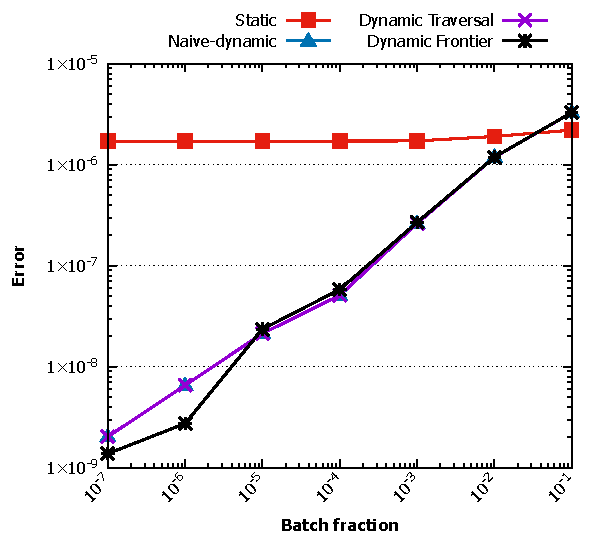
\includegraphics[width=0.38\linewidth]{out/deletions-error-mean.pdf}
  }
  \subfigure[Results on each graph]{
    \label{fig:deletions-error--all}
    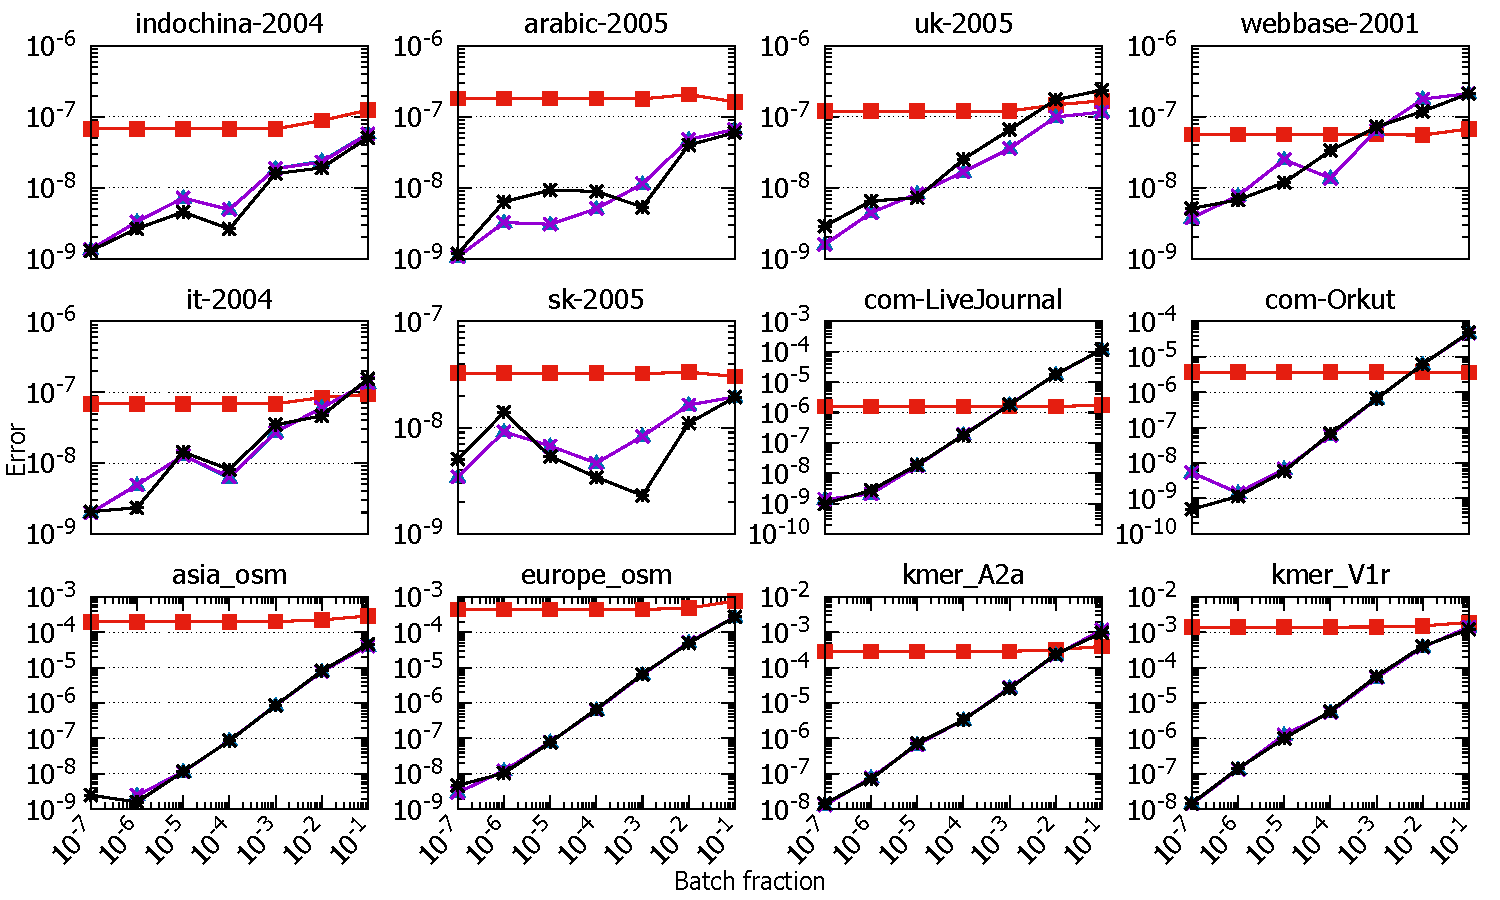
\includegraphics[width=0.58\linewidth]{out/deletions-error-all.pdf}
  } \\[-1ex]
  \caption{Deletions Time taken (solid lines), and modularity of communities obtained (dashed lines) along the Y2 axis, with X, X, and X (Algorithm X) on batch updates of increasing size from $10^{-7} |E|$ to $0.1 |E|$. Note that both axes are logarithmic. The numbers on the lines corresponding to X and X indicate the error of X over  the two algorithms, respectively.}
  \label{fig:deletions-error}
\end{figure*}

\begin{figure*}[hbtp]
  \centering
  % \includegraphics[width=0.44\linewidth]{out/8020-runtime-key.pdf}
  \subfigure[Overall result]{
    \label{fig:8020-runtime--mean}
    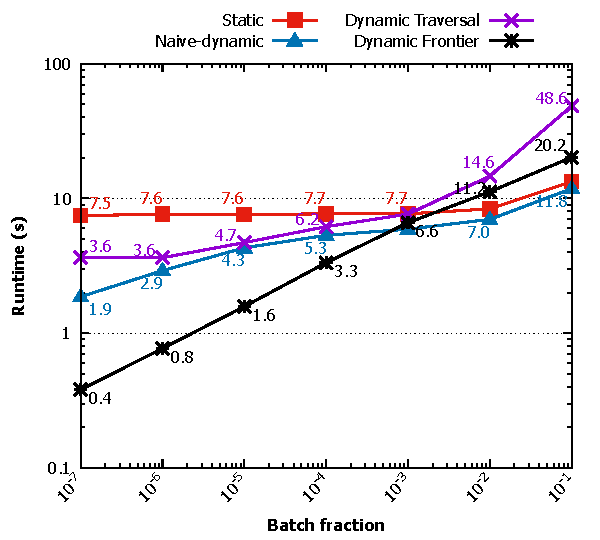
\includegraphics[width=0.38\linewidth]{out/8020-runtime-mean.pdf}
  }
  \subfigure[Results on each graph]{
    \label{fig:8020-runtime--all}
    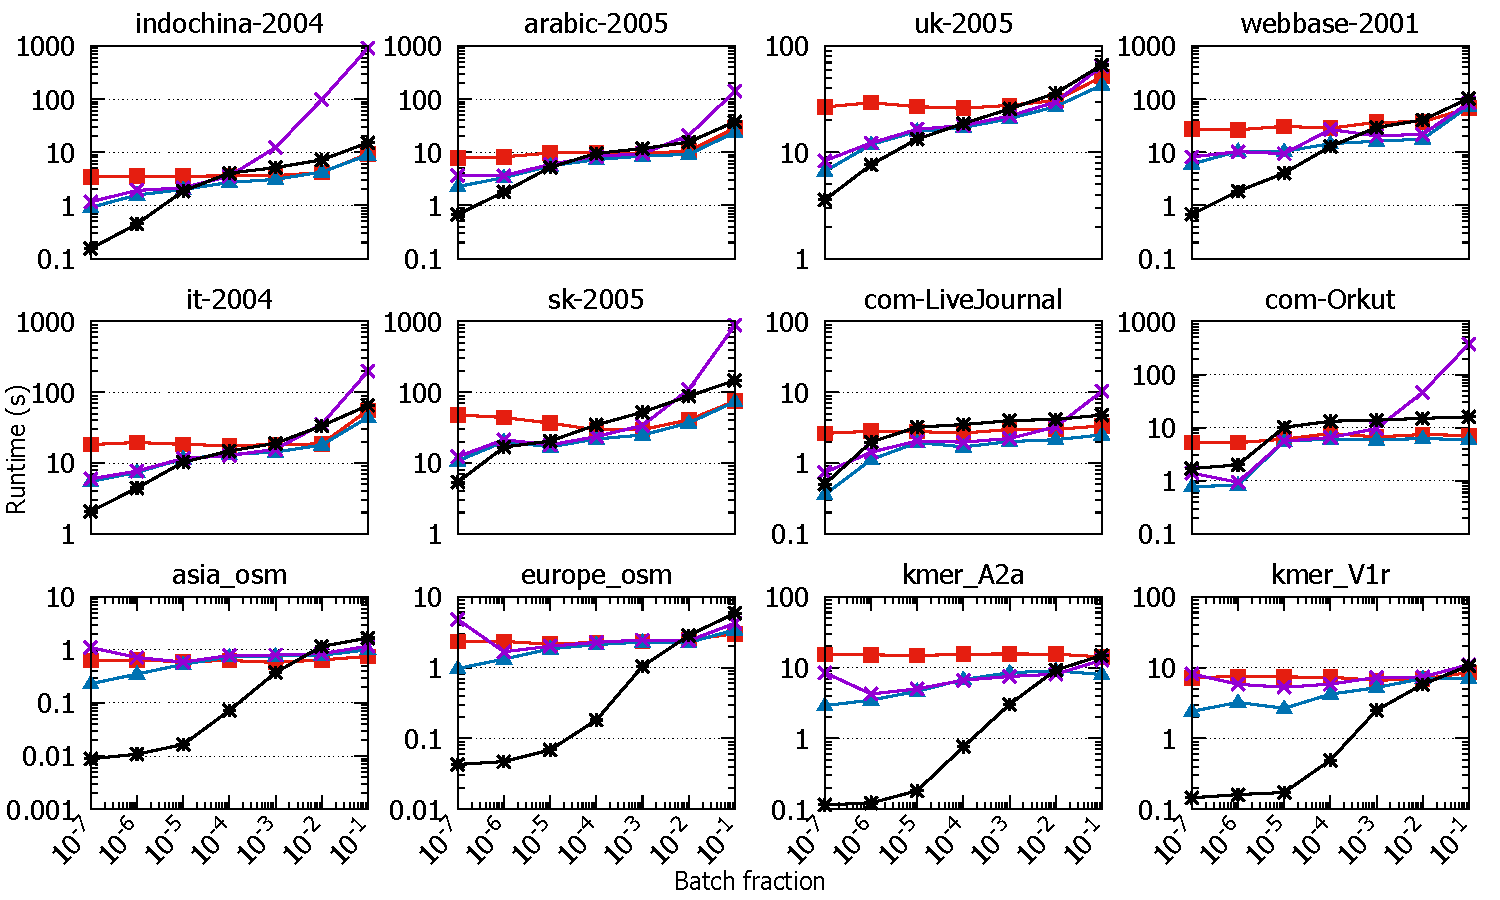
\includegraphics[width=0.58\linewidth]{out/8020-runtime-all.pdf}
  } \\[-1ex]
  \caption{8020 Time taken (solid lines), and modularity of communities obtained (dashed lines) along the Y2 axis, with X, X, and X (Algorithm X) on batch updates of increasing size from $10^{-7} |E|$ to $0.1 |E|$. Note that both axes are logarithmic. The numbers on the lines corresponding to X and X indicate the speedup of X over  the two algorithms, respectively.}
  \label{fig:8020-runtime}
\end{figure*}

\begin{figure*}[hbtp]
  \centering
  % \includegraphics[width=0.44\linewidth]{out/8020-speedup-key.pdf}
  \subfigure[Overall result]{
    \label{fig:8020-speedup--mean}
    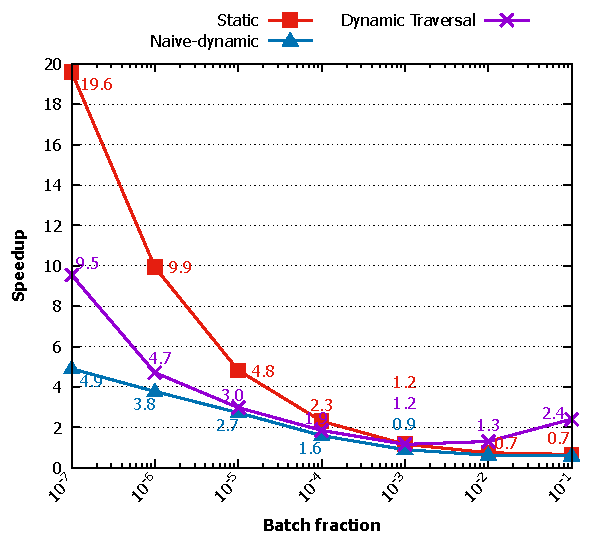
\includegraphics[width=0.38\linewidth]{out/8020-speedup-mean.pdf}
  }
  \subfigure[Results on each graph]{
    \label{fig:8020-speedup--all}
    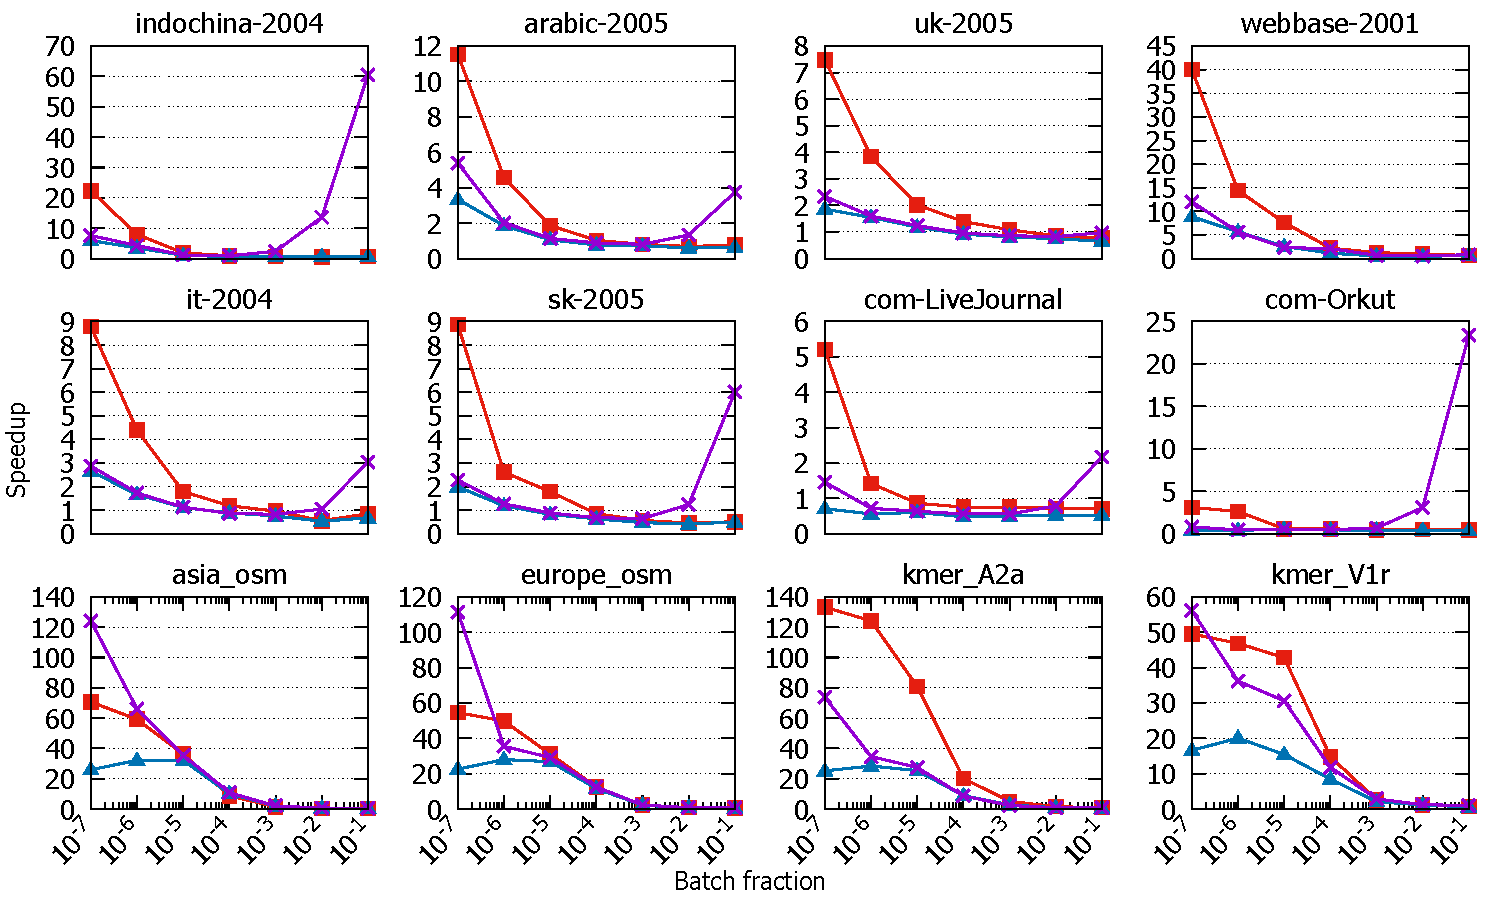
\includegraphics[width=0.58\linewidth]{out/8020-speedup-all.pdf}
  } \\[-1ex]
  \caption{8020 Time taken (solid lines), and modularity of communities obtained (dashed lines) along the Y2 axis, with X, X, and X (Algorithm X) on batch updates of increasing size from $10^{-7} |E|$ to $0.1 |E|$. Note that both axes are logarithmic. The numbers on the lines corresponding to X and X indicate the speedup of X over  the two algorithms, respectively.}
  \label{fig:8020-speedup}
\end{figure*}

\begin{figure*}[hbtp]
  \centering
  % \includegraphics[width=0.44\linewidth]{out/8020-error-key.pdf}
  \subfigure[Overall result]{
    \label{fig:8020-error--mean}
    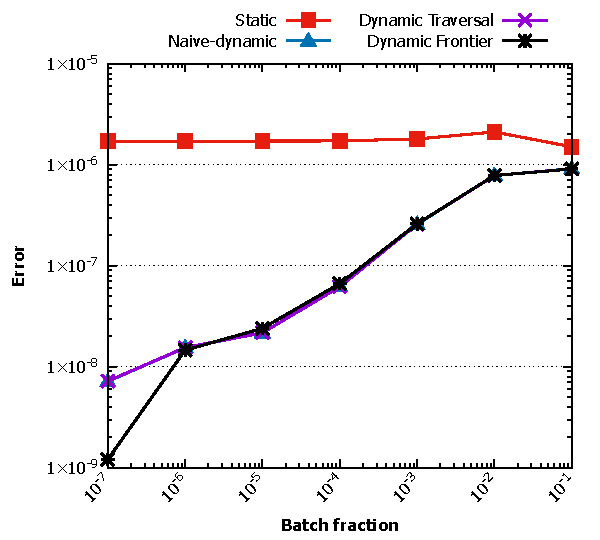
\includegraphics[width=0.38\linewidth]{out/8020-error-mean.pdf}
  }
  \subfigure[Results on each graph]{
    \label{fig:8020-error--all}
    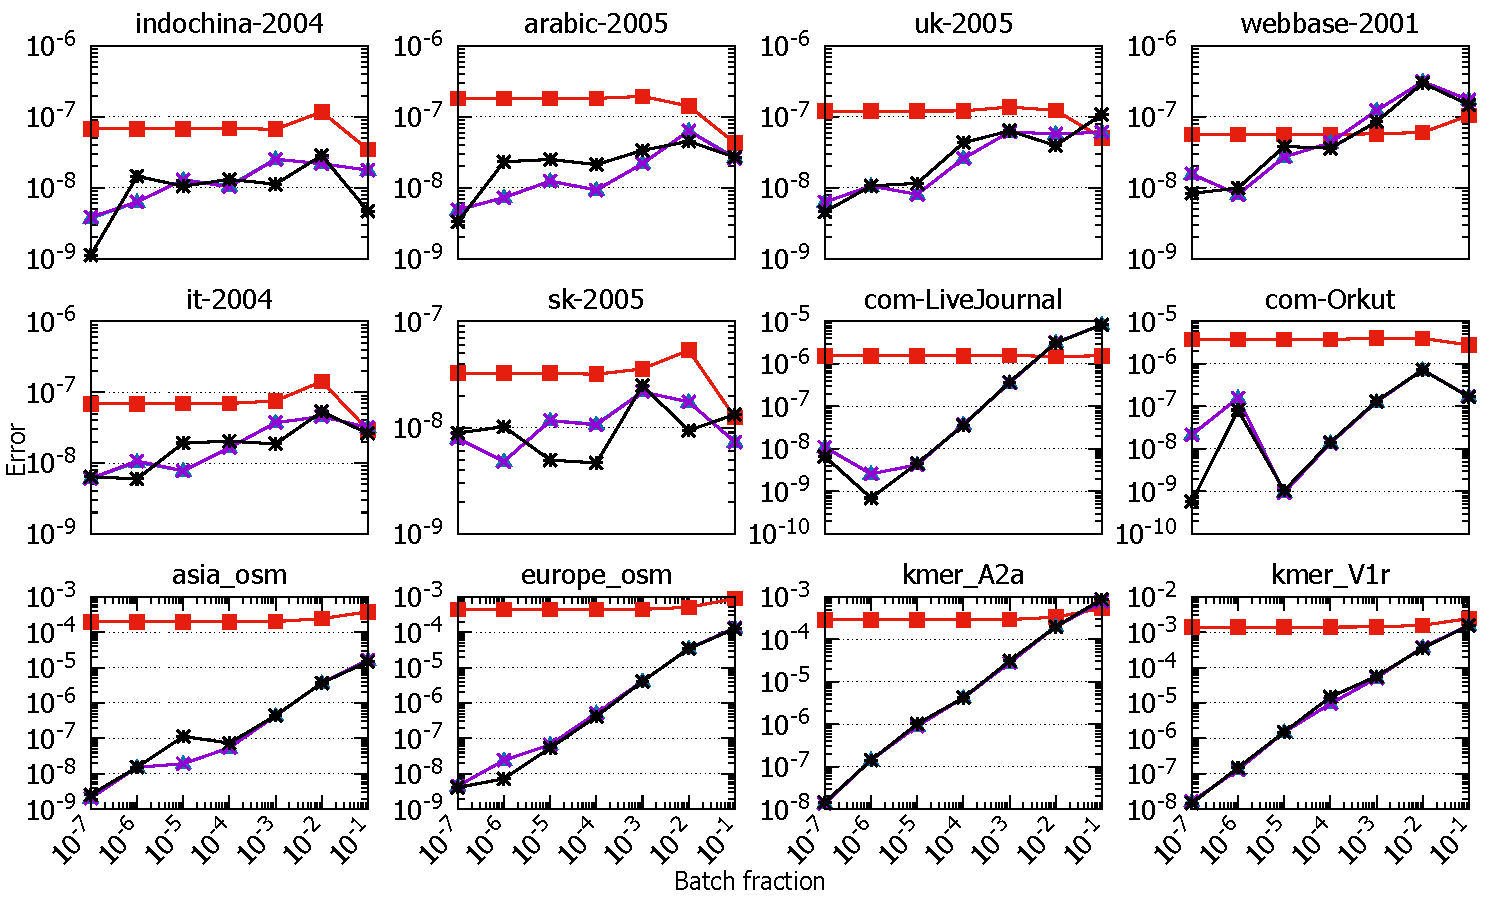
\includegraphics[width=0.58\linewidth]{out/8020-error-all.pdf}
  } \\[-1ex]
  \caption{Error comparison of \textit{Static}, \textit{Naive-dynamic}, \textit{Dynamic Traversal}, and \textit{Dynamic Frontier} PageRank with respect to a Reference Static PageRank (with a tolerance $\tau$ of $10^{-100}$ and limited to $500$ iterations), using $L1$-norm. Batch updates range from $10^{-7} |E|$ to $0.1 |E|$ (logarithmic scale), consisting of $80\%$ edge insertions and $20\%$ edge deletions to simulate realistic dynamic graph updates. The right figure depicts the error for each approach in relation to each graph, while the left figure showcases overall errors using geometric mean for consistent scaling across graphs.}
  \label{fig:8020-error}
\end{figure*}





\paragraph{Accuracy of DF-PageRank}

The error with respect to reference PageRank for \FroBarf{} (as well as \FroWbar{}), as shown in Figure \ref{fig:no-failure-am-error}, starts increasing from $5\times10^{-10}$ to $9\times10^{-10}$ at a batch size of $10^{-6} |E|$ to $10^{-4} |E|$, and then drops back at a batch size of $10^{-2} |E|$. \textit{Dynamic Frontier} approach picks only outgoing neighbors of those vertices to mark whose rank changes by at least a frontier tolerance of $\tau' = \tau/1000$ (where tolerance $\tau = 10^{-10}$). The error falls back because most vertices are getting marked as affected with increasing batch size.  Note that the error with \FroBarf{} lies within the acceptable range of $[0, 10^{-9})$ for a tolerance of $\tau = 10^{-10}$. There is no extra overhead introduced by our barrier-free approach in the absence of faults.
% Note that the slowdown of the \textit{Static} PageRank at a batch size of $0.1 |E|$ can be attributed to the difference in the size of the modified graph. This is because \textit{Dynamic Frontier} approach misses to mark some vertices as affected.

% \input{src/fig-fault-none}



\subsection{Comparing Performance of DF-PageRank}

\subsection{Analyzing Performance of DF-PageRank}

Task-wise split of DF-PageRank with varying batch sizes.

\subsection{Strong Scaling of DF-PageRank}

We next study the strong-scaling behavior of \FroWbar{} and \FroBarf{} on batch updates of a fixed size of $10^{-4} |E|$ in the absence of faults. Here, we measure the speedup of each algorithm with an increasing number of threads from $1$ to $64$ in multiples of $2$ with respect to a single-threaded execution of the algorithm. We additionally compare \StaWbar{}, \StaBarf{}, \NaiWbar{}, and \NaiBarf{}.

We observe from Figure \ref{fig:strong-scaling} that all algorithms exhibit a good decrease in their run time over increasing number of threads. With $64$ threads, \StaBarf{}, \NaiBarf{}, and \FroBarf{} offers an average speedup of $21\times$, while \StaWbar{}, \NaiWbar{}, and \FroWbar{} offer an average speedup of $15\times$ over a single thread.
% Thus, \FroBarf{} offers good scaling performance.


\subsection{Weak Scaling of DF-PageRank}

\subsection{Behavior of DF-PageRank on Temporal Graphs}
